In the previous sections, we have been covering the documentation and graphing of the software code, but in a large project, we may also need to document and visualize the CMake code as well. The relations between CMake targets may be complex, and this may render keeping track of all the dependencies hard. Fortunately, CMake can again help with this by providing a graph showing all dependencies between targets. By calling cmake -{}-graphviz=my-project.dot /path/to/build/dir, CMake will create files in the DOT language that contain how targets depend on each other.

The DOT language is a description language for graphs and can be interpreted by a multitude of programs, the most famous one being the freely available Graphviz. DOT files can be converted to images or even Portable Document Format (PDF) files using the dot command-line utility from Graphviz, like this: dot -Tpng filename.dot -o out.png.

Running these commands for the example project of this chapter will produce an output similar to this:

\begin{center}
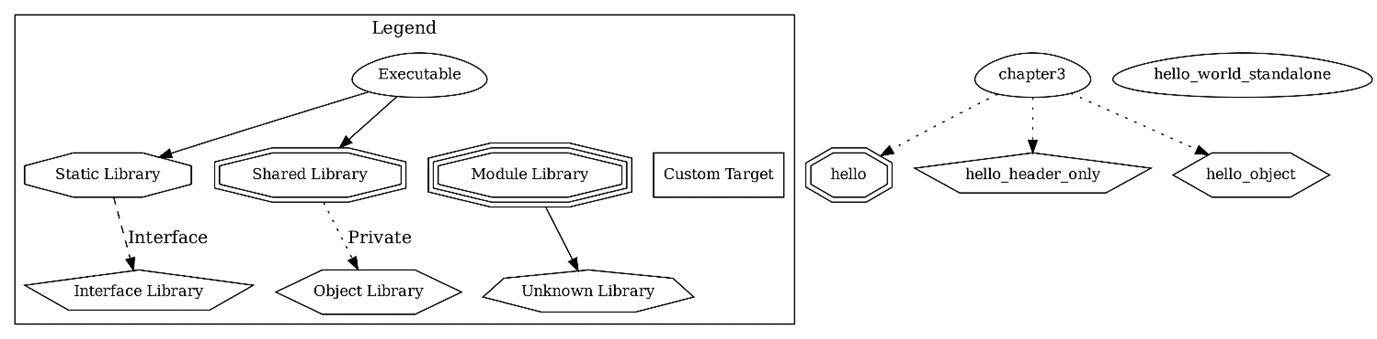
\includegraphics[width=0.8\textwidth]{content/2/chapter6/images/7.jpg}\\
Figure 6.7 – The project structure of chapter3 visualized with the DOT language
\end{center}

Behavior and options can be controlled by the variables provided in CMakeGraphVizOptions. When creating DOT graphs, CMake will look for a file called CMakeGraphVizOptions.cmake in the PROJECT\_SOURCE\_DIR and PROJECT\_BINARY\_DIR directories and, if found, will use the values provided within. An example of such a config file might look like this:

\begin{lstlisting}[style=styleCMake]
set(GRAPHVIZ_GRAPH_NAME "CMake Best Practices")
set(GRAPHVIZ_GENERATE_PER_TARGET FALSE)
set(GRAPHVIZ_GENERATE_DEPENDERS FALSE)
\end{lstlisting}

By default, CMake creates dependency graphs for all targets. Setting GRAPHVIZ\_GENERATE\_PER\_TARGET and GRAPHVIZ\_GENERATE\_DEPENDERS to FALSE will reduce the number of files generated. A full set of available options can be found in the CMake documentation at \url{https://cmake.org/cmake/help/latest/module/CMakeGraphVizOptions.html}.

















